\chapter{Surfaces, adsorption et catalyse hétérogène}\label{ch:b3:surfaces-catalysis}

Sous une voiture, dans une enveloppe d'acier, se trouve un nid d'abeilles
en céramique dont les milliers de canaux sont revêtus d'un oxyde poreux
portant quelques grammes de platine, de palladium et de rhodium. En une
fraction de seconde, les gaz d'échappement qui le traversent perdent
l'essentiel de leur monoxyde de carbone, de leurs hydrocarbures imbrûlés
et de leurs oxydes d'azote. Rien ne se passe dans le gaz~: chacune de
ces réactions a lieu à la surface des particules de métal, larges de
quelques nanomètres. La plus grande partie de l'industrie chimique
fonctionne de la même façon, de l'ammoniac des engrais au craquage du
pétrole. Ce chapitre décrit comment les molécules se fixent sur les
surfaces, quelle part d'une surface elles recouvrent, comment se
déroulent les réactions de surface, et comment un catalyseur solide est
fabriqué, mesuré et observé.

\begin{recall}
Le volume de première année a défini les catalyseurs et la différence
entre catalyse homogène et catalyse hétérogène, et a décrit
l'empilement cubique à faces centrées des métaux. Le volume de deuxième
année a défini le taux de conversion, la sélectivité et la fréquence de
cycles d'un catalyseur, ainsi que le principe de Le Chatelier. Le
\Cref{ch:b3:x-ray-diffraction} a introduit les \omterm{def:b3:x-ray-diffraction:miller}{indices de Miller}, le
\cref{ch:b3:rate-theories} l'\omterm{thm:b3:rate-theories:eyring}{équation d'Eyring} et le
\cref{ch:b3:partition-functions} la statistique des distributions.
\end{recall}

\begin{omfigure}
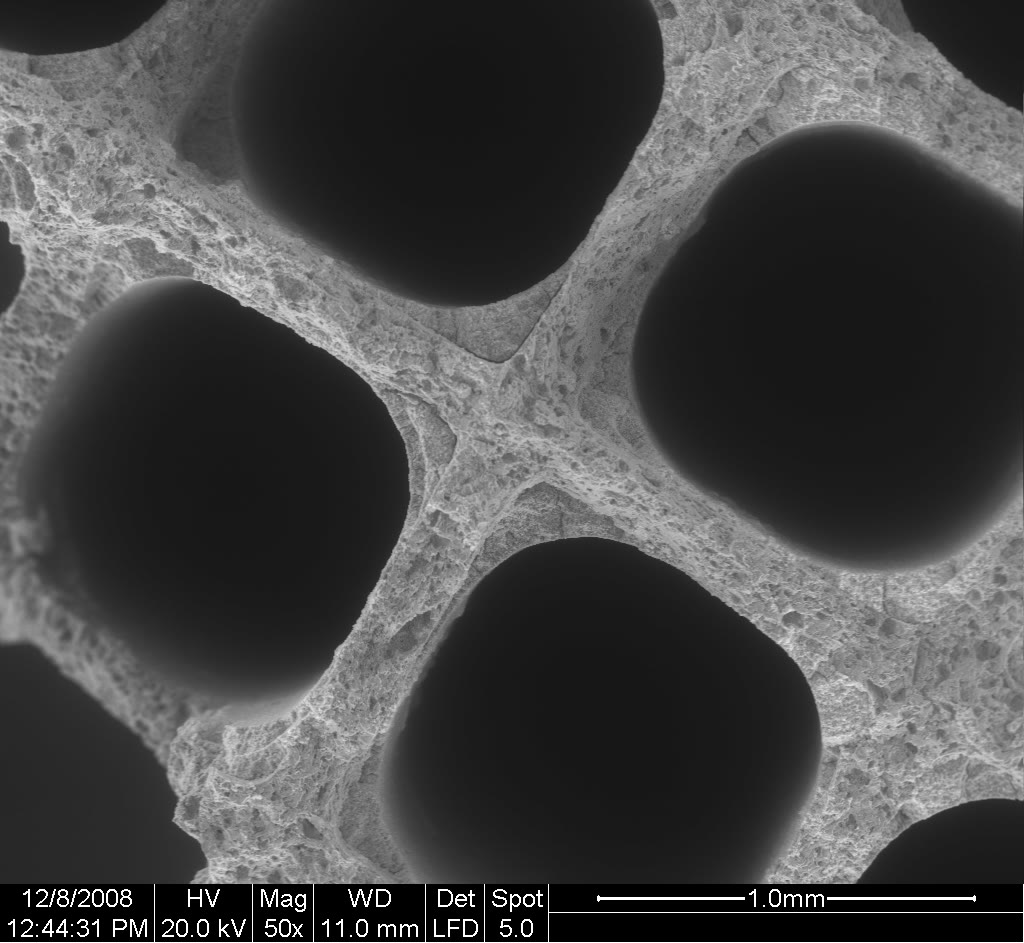
\includegraphics[width=0.48\linewidth]{images/book4/converter-sem.jpg}

{\small Le nid d'abeilles céramique d'un pot catalytique vu au microscope
électronique à balayage (barre d'échelle \qty{1.0}{mm})~: des canaux
carrés séparés par de minces parois poreuses, qui portent le revêtement
d'oxyde et ses particules de métal.}
\end{omfigure}

\section{L'adsorption}

\begin{definition}[Adsorption]\label{def:b3:surfaces-catalysis:adsorption}
L'\emph{adsorption}\index{adsorption} est l'accumulation de molécules d'un
gaz ou d'un soluté à la surface d'un solide ou d'un liquide. La molécule
qui s'adsorbe est l'\emph{adsorbat}\index{adsorbat}, le solide
l'\emph{adsorbant}\index{adsorbant}~;
le processus inverse est la \emph{désorption}\index{desorption@désorption}.
\end{definition}

\begin{definition}[Physisorption, chimisorption]\label{def:b3:surfaces-catalysis:physi-chemi}
La \emph{physisorption}\index{physisorption} est une \omterm{def:b3:surfaces-catalysis:adsorption}{adsorption} due aux
forces de van der Waals, avec des enthalpies d'\omterm{def:b3:surfaces-catalysis:adsorption}{adsorption} de quelques
dizaines de kilojoules par mole au plus, comparables aux enthalpies de
condensation, et sans modification de la molécule. La
\emph{chimisorption}\index{chimisorption} forme des liaisons chimiques
avec la surface, avec des enthalpies d'environ 40 à plusieurs centaines
de kilojoules par mole~; elle peut rompre la molécule (chimisorption
dissociative) et s'arrête à une seule couche.
\end{definition}

\begin{omfigure}
\begin{tikzpicture}[font=\small, >=Stealth, x=1cm, y=1cm]
  \draw[->] (0,-2.6) -- (0,1.8) node[anchor=south] {énergie};
  \draw[->] (0,0) -- (8.0,0) node[anchor=south east] {distance à la surface};
  \draw[omDef, thick] plot[smooth, tension=0.7] coordinates {(1.6,1.6) (2.2,-0.25) (2.8,-0.62) (3.6,-0.35) (5.0,-0.08) (7.5,0)};
  \draw[omThm, thick] plot[smooth, tension=0.6] coordinates {(0.45,1.6) (0.8,-1.2) (1.2,-2.2) (1.7,-1.6) (2.35,-0.15) (2.9,0.9) (3.5,1.5)};
  \node[omDef, anchor=north west, font=\scriptsize] at (3.4,-0.4) {\ce{H2} physisorbé (précurseur)};
  \node[omThm, anchor=west, font=\scriptsize] at (1.75,-1.9) {2 H chimisorbés};
  \node[omThm, anchor=west, font=\scriptsize, align=left] at (3.55,1.45) {vers $\mathrm{H} + \mathrm{H}$\\ loin de la surface};
  \fill (2.3,-0.2) circle (1.5pt);
  \node[font=\scriptsize] (cr) at (1.25,0.55) {\tiny croisement};
  \draw[black!60] (cr.south east) -- (2.27,-0.15);
\end{tikzpicture}

{\small Énergie potentielle d'une molécule de dihydrogène qui s'approche
d'une surface métallique (schéma). La molécule tombe d'abord dans le puits
peu profond de la \omterm{def:b3:surfaces-catalysis:physi-chemi}{physisorption}~; là où cette courbe croise celle de deux
atomes H liés séparément, elle peut se dissocier vers le puits profond
de la \omterm{def:b3:surfaces-catalysis:physi-chemi}{chimisorption}. Si le croisement se situe au-dessus de zéro, la
\omterm{def:b3:surfaces-catalysis:physi-chemi}{chimisorption} dissociative est activée.}
\end{omfigure}

Les surfaces des particules métalliques exposent surtout les faces les
plus denses du réseau cubique à faces centrées, (111) et (100). Un
\omterm{def:b3:surfaces-catalysis:adsorption}{adsorbat} peut s'y placer au-dessus d'un atome (site sommet), entre deux
atomes (site ponté) ou dans un creux entre trois ou quatre atomes (site
creux), et l'énergie de liaison diffère d'un site à l'autre.

\begin{omfigure}
\begin{tikzpicture}[font=\scriptsize]
  % fcc(111): hexagonal layer, spacing 0.6 cm
  \foreach \i in {0,...,5}{\foreach \j in {0,...,4}{
    \shade[ball color=black!25] ({0.6*\i+0.3*\j},{0.52*\j}) circle (0.29);}}
  \fill[omThm] (1.2+0.3*1,0.52) circle (0.07);
  \fill[omDef] ({0.6*2+0.3*2+0.3},{0.52*2}) circle (0.07);
  \fill[black] ({0.6*3+0.3*2+0.3},{0.52*2+0.17}) circle (0.07);
  \fill[black!60!green] ({0.6*1+0.3*3+0.3},{0.52*3-0.17}) circle (0.07);
  \node[anchor=north] at (2.1,-0.45) {cfc(111)};
  % fcc(100): square layer
  \begin{scope}[xshift=5.6cm]
  \foreach \i in {0,...,4}{\foreach \j in {0,...,4}{
    \shade[ball color=black!25] ({0.6*\i},{0.6*\j}) circle (0.29);}}
  \fill[omThm] (1.2,1.2) circle (0.07);
  \fill[omDef] (1.5,1.8) circle (0.07);
  \fill[black] (2.1,0.9) circle (0.07);
  \node[anchor=north] at (1.2,-0.45) {cfc(100)};
  \end{scope}
  \node[anchor=west, align=left] at (9.0,1.6) {\textcolor{omThm}{$\bullet$} sommet\\ \textcolor{omDef}{$\bullet$} ponté\\
    $\bullet$ creux (d'ordre 3 ou 4)\\ \textcolor{black!60!green}{$\bullet$} second creux d'ordre 3 (111)};
\end{tikzpicture}

{\small Vues de dessus des deux faces les plus denses d'un métal cubique
à faces centrées, avec les sites d'\omterm{def:b3:surfaces-catalysis:adsorption}{adsorption}~: au sommet d'un atome, en
pont entre deux, et dans les creux entre trois atomes sur (111) (de deux
sortes, au-dessus d'un atome de la deuxième couche ou non) ou entre
quatre atomes sur (100).}
\end{omfigure}

\begin{definition}[Taux de recouvrement, monocouche]\label{def:b3:surfaces-catalysis:coverage}
Le \emph{taux de recouvrement}\index{taux de recouvrement} $\theta$ d'une
surface est la fraction de ses sites d'\omterm{def:b3:surfaces-catalysis:adsorption}{adsorption} qui sont occupés. Une
\emph{monocouche}\index{monocouche} est une couche unique et complète
d'\omterm{def:b3:surfaces-catalysis:adsorption}{adsorbat}, $\theta = 1$.
\end{definition}

\section{Isothermes}

\begin{theorem}[Isotherme de Langmuir]\label{thm:b3:surfaces-catalysis:langmuir}
Si une surface possède des sites identiques et indépendants, chacun
retenant une molécule, le \omterm{def:b3:surfaces-catalysis:coverage}{taux de recouvrement} à l'équilibre avec un gaz
sous la pression $p$ vaut
\[
  \theta = \frac{Kp}{1 + Kp},
\]
où $K$, la constante d'équilibre d'\omterm{def:b3:surfaces-catalysis:adsorption}{adsorption}, ne dépend que de la
température. C'est l'\emph{isotherme de Langmuir}\index{isotherme de Langmuir}.
\end{theorem}

\begin{proof}
Démonstration cinétique. Les molécules s'adsorbent sur les sites libres à
la vitesse $k_ap(1 - \theta)N$ ($N$
sites) et se désorbent à la vitesse $k_d\theta N$. À l'équilibre, les
deux sont égales~: $\theta/(1 - \theta)
= (k_a/k_d)p$, ce qui donne le résultat avec $K = k_a/k_d$.

Démonstration statistique. $M$ molécules peuvent se disposer sur $N$
sites de $N!/(M!(N - M)!)$ façons,
chaque molécule adsorbée ayant une fonction de partition interne
$q_{\mathrm s}$ (ses vibrations contre la surface et son énergie de
liaison). Avec la formule de Stirling,
le potentiel chimique des molécules adsorbées vaut $\mu_{\mathrm s} = -kT\ln\bigl(q_{\mathrm s}\frac{1 - \theta}{\theta}\bigr)$~;
celui du gaz parfait vaut $\mu_{\mathrm g} = \mu_{\mathrm g}^\circ + kT\ln(p/p^\circ)$. L'équilibre, $\mu_{\mathrm s} = \mu_{\mathrm g}$, donne
$\theta/(1 - \theta) = q_{\mathrm s}\eu^{\mu_{\mathrm g}^\circ/kT}p/p^\circ$~:
la même loi, avec $K$ exprimée à l'aide de fonctions de partition.
\end{proof}

À basse pression, $\theta \approx Kp$ (régime de Henry)~; à haute
pression, $\theta \to 1$. Le \omterm{def:b3:surfaces-catalysis:coverage}{taux de recouvrement} vaut un demi pour
$p = 1/K$.

\begin{proposition}[Adsorption dissociative]\label{prop:b3:surfaces-catalysis:dissociative}
Pour un gaz diatomique qui se dissocie sur deux sites, $\mathrm{H_2} + 2\,{*} \to 2\,\mathrm{H}{*}$
(${*}$~: un site libre),
\[
  \theta = \frac{(Kp)^{1/2}}{1 + (Kp)^{1/2}},
\]
de sorte que $\theta \propto \sqrt p$ à basse pression.
\end{proposition}

\begin{proof}
L'\omterm{def:b3:surfaces-catalysis:adsorption}{adsorption} exige deux sites libres, à la vitesse $k_ap(1 - \theta)^2$~;
la \omterm{def:b3:surfaces-catalysis:adsorption}{désorption} exige que deux atomes adsorbés se recombinent, à la
vitesse $k_d\theta^2$. L'égalité donne $\theta/(1 - \theta) =
(Kp)^{1/2}$.
\end{proof}

\begin{proposition}[Adsorption compétitive]\label{prop:b3:surfaces-catalysis:competitive}
Deux gaz A et B en compétition pour les mêmes sites les recouvrent avec
\[
  \theta_{\mathrm A} = \frac{K_{\mathrm A}p_{\mathrm A}}{1 + K_{\mathrm A}p_{\mathrm A} + K_{\mathrm B}p_{\mathrm B}}, \qquad
  \theta_{\mathrm B} = \frac{K_{\mathrm B}p_{\mathrm B}}{1 + K_{\mathrm A}p_{\mathrm A} + K_{\mathrm B}p_{\mathrm B}} .
\]
\end{proposition}

\begin{proof}
Pour chaque gaz, $k_{a,\mathrm A}p_{\mathrm A}(1 - \theta_{\mathrm A} - \theta_{\mathrm B}) = k_{d,\mathrm A}\theta_{\mathrm A}$
et de même pour B. Donc
$\theta_{\mathrm A} = K_{\mathrm A}p_{\mathrm A}\theta_\ast$ et $\theta_{\mathrm B} = K_{\mathrm B}p_{\mathrm B}\theta_\ast$
avec $\theta_\ast = 1 - \theta_{\mathrm A} - \theta_{\mathrm B}$ la fraction
libre~; en additionnant,
$1 - \theta_\ast = \theta_\ast(K_{\mathrm A}p_{\mathrm A} + K_{\mathrm B}p_{\mathrm B})$.
\end{proof}

\begin{definition}[Enthalpie isostérique d'adsorption]\label{def:b3:surfaces-catalysis:isosteric}
L'\emph{enthalpie isostérique d'adsorption}\index{enthalpie isosterique d'adsorption@enthalpie isostérique d'adsorption}
$\Delta_{\mathrm{ads}}H$ est l'enthalpie molaire d'\omterm{def:b3:surfaces-catalysis:adsorption}{adsorption} à \omterm{def:b3:surfaces-catalysis:coverage}{taux de
recouvrement} fixé, obtenue à partir des pressions qui donnent le même
\omterm{def:b3:surfaces-catalysis:coverage}{taux de recouvrement} à différentes températures.
\end{definition}

\begin{proposition}[Enthalpie isostérique]\label{prop:b3:surfaces-catalysis:isosteric}
À \omterm{def:b3:surfaces-catalysis:coverage}{taux de recouvrement} constant,
\[
  \Bigl(\frac{\partial\ln p}{\partial T}\Bigr)_\theta = -\frac{\Delta_{\mathrm{ads}}H}{RT^2} .
\]
\end{proposition}

\begin{proof}
À $\theta$ constant, $Kp$ est constant (pour une surface de Langmuir~;
en général, le même raisonnement vaut avec la constante d'équilibre à ce
\omterm{def:b3:surfaces-catalysis:coverage}{taux de recouvrement}), donc $\ln p =
\text{cste} - \ln K$. D'après la relation de van 't Hoff,
$\dd\ln K/\dd T = \Delta_{\mathrm{ads}}H/RT^2$ ($K$ étant
rapportée à une pression standard).
\end{proof}

Comme l'\omterm{def:b3:surfaces-catalysis:adsorption}{adsorption} est exothermique, des températures plus élevées
exigent des pressions plus élevées pour le même \omterm{def:b3:surfaces-catalysis:coverage}{taux de recouvrement}~:
les isothermes de la figure s'abaissent quand $T$ augmente.

\begin{theorem}[Isotherme BET]\label{thm:b3:surfaces-catalysis:bet}
Si les molécules s'adsorbent en couches successives, la première avec
une constante de liaison caractéristique de la surface et les suivantes
avec l'équilibre de condensation du liquide, la quantité adsorbée à la
pression relative $x = p/p^*$ ($p^*$~: pression de vapeur saturante de
l'\omterm{def:b3:surfaces-catalysis:adsorption}{adsorbat} liquide) vaut
\[
  \frac{v}{v_{\mathrm m}} = \frac{cx}{(1 - x)(1 - x + cx)},
\]
où $v_{\mathrm m}$ est la quantité d'une \omterm{def:b3:surfaces-catalysis:coverage}{monocouche} et $c$ une constante
liée à la différence entre l'enthalpie d'\omterm{def:b3:surfaces-catalysis:adsorption}{adsorption} dans la première
couche et l'enthalpie de condensation. C'est l'\emph{isotherme
BET}\index{isotherme BET} (Brunauer, Emmett et Teller).
\end{theorem}

\begin{proof}
Soit $s_i$ la fraction de la surface recouverte par exactement $i$
couches. Le bilan de chaque couche, comme dans la démonstration de
Langmuir, donne $s_1 = cxs_0$ et $s_i =
xs_{i-1}$ pour $i \ge 2$, donc $s_i = cx^is_0$. La quantité adsorbée vaut $v/v_{\mathrm m} =
\sum_iis_i/\sum_is_i$. Avec $\sum_{i\ge1}x^i = x/(1 - x)$ et $\sum_{i\ge1}ix^i = x/(1 - x)^2$~:
\[
  \frac{v}{v_{\mathrm m}} = \frac{cs_0\,x/(1 - x)^2}{s_0[1 + cx/(1 - x)]} = \frac{cx}{(1 - x)(1 - x + cx)} .
\]
\end{proof}

Sous forme réarrangée, $\dfrac{x}{v(1 - x)} = \dfrac{1}{v_{\mathrm m}c} + \dfrac{c - 1}{v_{\mathrm m}c}\,x$~:
une droite dont la pente et l'ordonnée à l'origine donnent
$v_{\mathrm m}$ et $c$, en général valable pour $0.05 < x < 0.30$.

\begin{definition}[Surface spécifique]\label{def:b3:surfaces-catalysis:surface-area}
La \emph{surface spécifique}\index{surface specifique@surface spécifique} d'un solide est son aire
par unité de masse, parois de ses pores comprises.
\end{definition}

\begin{method}[Surface spécifique à partir d'une isotherme de diazote]\label{met:b3:surfaces-catalysis:bet-area}
\begin{enumerate}
  \item Dégazer l'échantillon sous vide en le chauffant~; le refroidir
        dans l'azote liquide
        (\qty{77}{K}).
  \item Mesurer le volume de diazote adsorbé (ramené aux conditions
        normales) à des pressions relatives comprises entre 0.05 et 0.30.
  \item Tracer $x/(v(1 - x))$ en fonction de $x$~; de la pente et de
        l'ordonnée à l'origine,
        $v_{\mathrm m} = 1/(\text{pente} + \text{ordonnée})$ et $c = 1 + \text{pente}/\text{ordonnée}$.
  \item Aire $= n_{\mathrm m}N_Aa_{\mathrm m}$, avec $n_{\mathrm m}$ la
        quantité de la \omterm{def:b3:surfaces-catalysis:coverage}{monocouche} et $a_{\mathrm m} = \qty{0.162}{nm^2}$
        l'aire conventionnelle d'une molécule de diazote adsorbée.
\end{enumerate}
\end{method}

\begin{omfigure}
\begin{tikzpicture}
\begin{axis}[name=la, width=0.31\linewidth, height=5.0cm, xmin=0, xmax=100, ymin=0, ymax=1.05,
  axis lines=left, xlabel={$p$ / kPa}, ylabel={$\theta$}, tick label style={font=\small},
  label style={font=\small}, title={\small Langmuir}]
\addplot[omDef, thick] table[x=p_kPa, y=T300] {figdata/out/bachelor-3-langmuir-bet-langmuir.dat};
\addplot[omThm, thick] table[x=p_kPa, y=T350] {figdata/out/bachelor-3-langmuir-bet-langmuir.dat};
\node[font=\scriptsize, omDef, anchor=south east] at (axis cs:98,0.92) {\qty{300}{K}};
\node[font=\scriptsize, omThm, anchor=north east] at (axis cs:98,0.45) {\qty{350}{K}};
\end{axis}
\begin{axis}[name=be, at={(la.east)}, anchor=west, xshift=1.9cm, width=0.31\linewidth, height=5.0cm,
  xmin=0, xmax=0.9, ymin=0, ymax=200, axis lines=left, xlabel={$p/p^*$},
  ylabel={$v$ / \unit{cm^3.g^{-1}}}, tick label style={font=\small}, label style={font=\small},
  title={\small BET}]
\addplot[black, thick] table[x=x, y=v] {figdata/out/bachelor-3-langmuir-bet-bet.dat};
\addplot[only marks, mark=*, mark size=1.4pt, omDef] table[x=x, y=v] {figdata/out/bachelor-3-langmuir-bet-data.dat};
\draw[black!40, dashed] (axis cs:0,45) -- (axis cs:0.9,45);
\node[font=\scriptsize, anchor=south east] at (axis cs:0.88,45) {$v_{\mathrm m}$};
\end{axis}
\begin{axis}[at={(be.east)}, anchor=west, xshift=2.1cm, width=0.31\linewidth, height=5.0cm,
  xmin=0, xmax=0.35, ymin=0, ymax=0.0085, axis lines=left, xlabel={$x = p/p^*$},
  ylabel={$x/(v(1 - x))$}, tick label style={font=\small}, label style={font=\small},
  scaled y ticks=false, yticklabel style={/pgf/number format/fixed, /pgf/number format/precision=3},
  title={\small tracé BET}]
\addplot[black, thin] table[x=x, y=y] {figdata/out/bachelor-3-langmuir-bet-line.dat};
\addplot[only marks, mark=*, mark size=1.4pt, omDef] table[x=x, y=y] {figdata/out/bachelor-3-langmuir-bet-data.dat};
\end{axis}
\end{tikzpicture}

{\small À gauche~: \omterm{thm:b3:surfaces-catalysis:langmuir}{isothermes de Langmuir} d'une \omterm{def:b3:surfaces-catalysis:physi-chemi}{chimisorption} modèle
($\Delta_{\mathrm{ads}}H = \qty{-40}{kJ/mol}$) à
deux températures. Au milieu~: une \omterm{thm:b3:surfaces-catalysis:bet}{isotherme BET} (modèle,
$v_{\mathrm m} = \qty{45}{cm^3.g^{-1}}$, $c = 120$), avec les
points du problème du week-end~; les couches s'empilent et la quantité
diverge au voisinage de
$p = p^*$, où le gaz se condense. À droite~: le tracé BET linéaire des
mêmes points.}
\end{omfigure}

\section{Cinétique des réactions de surface}

\begin{definition}[Mécanismes de Langmuir--Hinshelwood et d'Eley--Rideal]\label{def:b3:surfaces-catalysis:mechanisms}
Dans le \emph{mécanisme de Langmuir--Hinshelwood}\index{mecanisme de Langmuir--Hinshelwood@mécanisme de Langmuir--Hinshelwood},
les deux réactifs sont adsorbés et réagissent à la surface~; dans le
\emph{mécanisme d'Eley--Rideal}\index{mecanisme d'Eley--Rideal@mécanisme d'Eley--Rideal}, un réactif
adsorbé réagit avec une molécule qui arrive de la phase gazeuse.
\end{definition}

\begin{proposition}[Vitesse de Langmuir--Hinshelwood]\label{prop:b3:surfaces-catalysis:lh-rate}
Si les équilibres d'\omterm{def:b3:surfaces-catalysis:adsorption}{adsorption} sont rapides et que la réaction de surface
entre A et B adsorbés est cinétiquement déterminante,
\[
  r = k\theta_{\mathrm A}\theta_{\mathrm B} = \frac{kK_{\mathrm A}p_{\mathrm A}K_{\mathrm B}p_{\mathrm B}}{(1 + K_{\mathrm A}p_{\mathrm A} + K_{\mathrm B}p_{\mathrm B})^2},
\]
qui, à $p_{\mathrm B}$ fixée, est maximale quand $K_{\mathrm A}p_{\mathrm A} = 1 + K_{\mathrm B}p_{\mathrm B}$
puis décroît à mesure que A chasse B de la surface.
\end{proposition}

\begin{proof}
Les \omterm{def:b3:surfaces-catalysis:coverage}{taux de recouvrement} sont ceux de la
\cref{prop:b3:surfaces-catalysis:competitive}. Avec $u =
K_{\mathrm A}p_{\mathrm A}$ et $a = 1 + K_{\mathrm B}p_{\mathrm B}$, $r \propto u/(a + u)^2$,
dont la dérivée $(a - u)/(a + u)^3$ s'annule pour
$u = a$.
\end{proof}

\begin{proposition}[Vitesse d'Eley--Rideal]\label{prop:b3:surfaces-catalysis:er-rate}
Si A adsorbé réagit avec B gazeux,
\[
  r = k\theta_{\mathrm A}p_{\mathrm B} = \frac{kK_{\mathrm A}p_{\mathrm A}p_{\mathrm B}}{1 + K_{\mathrm A}p_{\mathrm A}},
\]
qui croît avec $p_{\mathrm A}$ jusqu'à un palier, sans maximum.
\end{proposition}

\begin{proof}
B n'entre pas en compétition pour les sites~: $\theta_{\mathrm A}$ est le
\omterm{def:b3:surfaces-catalysis:coverage}{taux de recouvrement} de Langmuir de A seul, et la vitesse lui est
proportionnelle, ainsi qu'à la fréquence des collisions de B avec la
surface, proportionnelle à $p_{\mathrm B}$.
\end{proof}

\begin{method}[LH ou ER d'après la dépendance en pression]\label{met:b3:surfaces-catalysis:mechanism-from-rate}
\begin{enumerate}
  \item Mesurer la vitesse en fonction de la pression de chaque réactif,
        l'autre étant maintenue fixe.
  \item Un maximum, puis une décroissance (ordre négatif à haute
        pression)~: Langmuir--Hinshelwood, le réactif inhibant la
        réaction en occupant les sites.
  \item Une croissance jusqu'à un palier pour un réactif et un ordre 1
        pour l'autre à toutes les pressions~: Eley--Rideal.
  \item Confirmer par marquage isotopique ou par spectroscopie de
        surface~; la plupart des réactions catalytiques se révèlent de
        type Langmuir--Hinshelwood.
\end{enumerate}
\end{method}

\begin{omfigure}
\begin{tikzpicture}
\begin{axis}[width=0.6\linewidth, height=5.4cm, xmin=0, xmax=10, ymin=0, ymax=0.3,
  axis lines=left, xlabel={$p_{\mathrm A}$ (réduite)}, ylabel={vitesse (réduite)},
  tick label style={font=\small}, label style={font=\small},
  legend style={font=\scriptsize, draw=none, at={(1.03,0.98)}, anchor=north west}, legend cell align=left]
\addplot[omDef!50, thick] table[x=pA, y=pB05] {figdata/out/bachelor-3-surface-rates.dat};
\addplot[omDef, thick] table[x=pA, y=pB1] {figdata/out/bachelor-3-surface-rates.dat};
\addplot[black, thick] table[x=pA, y=pB3] {figdata/out/bachelor-3-surface-rates.dat};
\addplot[omThm, thick, dashed] table[x=pA, y=ER] {figdata/out/bachelor-3-surface-rates.dat};
\legend{{LH, $p_{\mathrm B} = 0.5$}, {LH, $p_{\mathrm B} = 1$}, {LH, $p_{\mathrm B} = 3$}, {ER ($\times\frac14$)}}
\end{axis}
\end{tikzpicture}

{\small Vitesses d'une réaction de surface bimoléculaire en fonction de la
pression de A (unités réduites, $K_{\mathrm A} = K_{\mathrm B} = 1$).
Langmuir--Hinshelwood~: chaque courbe passe par un maximum pour
$K_{\mathrm A}p_{\mathrm A} =
1 + K_{\mathrm B}p_{\mathrm B}$, puis décroît à mesure que A déplace B.
Eley--Rideal (en tirets, mise à l'échelle)~: un palier.}
\end{omfigure}

\begin{proposition}[Énergie d'activation apparente]\label{prop:b3:surfaces-catalysis:apparent-ea}
Pour une réaction de surface monomoléculaire avec \omterm{def:b3:surfaces-catalysis:adsorption}{adsorption} de Langmuir,
$r = k\theta = kKp/(1 + Kp)$.
À faible \omterm{def:b3:surfaces-catalysis:coverage}{taux de recouvrement}, l'énergie d'activation mesurée vaut
$E_{a,\mathrm{app}} = E_a + \Delta_{\mathrm{ads}}H$~; à fort \omterm{def:b3:surfaces-catalysis:coverage}{taux de
recouvrement}, elle vaut $E_a$.
\end{proposition}

\begin{proof}
À faible \omterm{def:b3:surfaces-catalysis:coverage}{taux de recouvrement}, $r \approx kKp$, donc $\dd\ln r/\dd T = \dd\ln k/\dd T + \dd\ln K/\dd T = (E_a + \Delta_{\mathrm{ads}}H)/RT^2$.
À fort \omterm{def:b3:surfaces-catalysis:coverage}{taux de recouvrement}, $\theta \approx 1$ et $r \approx k$.
\end{proof}

Comme $\Delta_{\mathrm{ads}}H < 0$, une réaction sur une surface peu
recouverte paraît plus facile que ne l'indique sa vraie barrière~:
élever la température accélère l'étape de surface, mais vide la
surface.

\begin{definition}[Principe de Sabatier, courbe en volcan]\label{def:b3:surfaces-catalysis:sabatier}
Le \emph{principe de Sabatier}\index{principe de Sabatier} énonce que le
meilleur catalyseur fixe les réactifs ni trop faiblement (ils ne
s'adsorbent pas ou ne sont pas activés) ni trop fortement (les produits
ne partent pas et bloquent les sites). Une
\emph{courbe en volcan}\index{courbe en volcan} donnant l'activité d'une
série de catalyseurs en fonction d'une énergie de liaison présente un
maximum pour une liaison intermédiaire.
\end{definition}

\begin{omfigure}
\begin{tikzpicture}[font=\small, >=Stealth]
  \draw[->] (0,0) -- (7.2,0) node[anchor=north east] {force de liaison de l'adsorbat};
  \draw[->] (0,0) -- (0,3.6) node[anchor=south] {activité};
  \draw[omDef, very thick] (0.4,0.3) -- (3.4,3.0) -- (6.6,0.4);
  \node[anchor=south, align=center, font=\scriptsize] at (1.35,2.0) {liaison trop faible~:\\ réactifs non\\ activés};
  \node[anchor=south, align=center, font=\scriptsize] at (5.9,2.0) {liaison trop forte~:\\ les produits\\ bloquent les sites};
  \node[anchor=south, font=\scriptsize] at (3.4,3.05) {meilleur catalyseur};
\end{tikzpicture}

{\small Une \omterm{def:b3:surfaces-catalysis:sabatier}{courbe en volcan} (qualitative)~: l'activité d'une série de
catalyseurs en fonction de la force avec laquelle ils fixent un
intermédiaire clé.}
\end{omfigure}

\section{Catalyseurs industriels}

\begin{definition}[Conception d'un catalyseur]\label{def:b3:surfaces-catalysis:catalyst-design}
Un \emph{support de catalyseur}\index{support de catalyseur} est un solide
poreux de grande surface (alumine, silice, carbone) qui porte de petites
particules de la phase active. Un
\emph{promoteur}\index{promoteur} est un additif, inactif seul, qui
augmente l'activité, la sélectivité ou la stabilité. Un \emph{poison de
catalyseur}\index{poison de catalyseur} est une substance qui se fixe
fortement sur les \omterm{def:b3:complex-kinetics:enzyme}{sites actifs} et les bloque.
La \emph{dispersion métallique}\index{dispersion metallique@dispersion métallique} $D$ est la fraction des atomes
de métal situés en surface. Le \emph{frittage}\index{frittage} est la
croissance des particules à haute température, qui diminue la
dispersion.
\end{definition}

\begin{method}[Dispersion et taille des particules par chimisorption du dihydrogène]\label{met:b3:surfaces-catalysis:dispersion}
\begin{enumerate}
  \item Réduire le catalyseur sous dihydrogène, faire le vide, et mesurer
        le volume de \ce{H2}
        chimisorbé (ramené aux conditions normales) sur le métal~; le
        support n'en adsorbe pas.
  \item Supposer un atome H par atome de métal de surface~: $D = n_{\ce{H}}/n_{\text{métal}}$.
  \item Pour des sphères de diamètre $d$, $D = 6(v_{\mathrm{at}}/a_{\mathrm{at}})/d$,
        avec $v_{\mathrm{at}}$ le volume par atome dans le
        massif et $a_{\mathrm{at}}$ l'aire par atome de surface~; donc $d = 6v_{\mathrm{at}}/(a_{\mathrm{at}}D)$.
\end{enumerate}
\end{method}

La synthèse de l'ammoniac, $\ce{N2 + 3 H2 <=> 2 NH3}$, se déroule vers
400 à \qty{500}{\celsius} et 100 à
\qty{300}{bar} sur du fer promu par l'oxyde de potassium et l'alumine~:
l'alumine empêche les cristallites de fer de fritter, le potassium
augmente l'activité. L'étape
cinétiquement déterminante est la \omterm{def:b3:surfaces-catalysis:physi-chemi}{chimisorption} dissociative de \ce{N2},
dont la triple liaison est la plus difficile à rompre. Quelque
150 millions de tonnes d'azote sont fixées ainsi chaque année.
% ledger: nh3:world-2024
L'oxydation de \ce{SO2} en \ce{SO3}, sur l'oxyde de vanadium(V) promu
par le sulfate de potassium, est l'étape clé de la fabrication de
l'acide sulfurique.

Le pot catalytique trois voies des moteurs à essence oxyde CO et les
hydrocarbures et réduit en même temps les oxydes d'azote, sur le platine
et le palladium (oxydation) et le rhodium (réduction de NO), dispersés
sur de l'alumine avec de l'oxyde de cérium, qui stocke et restitue le
dioxygène. Il ne fonctionne que dans une fenêtre étroite autour du
rapport air--carburant stœchiométrique~: avec un excès d'air, NO n'est
pas réduit~; avec un excès de carburant, CO n'est pas oxydé~; une sonde à
oxygène placée dans l'échappement maintient le moteur dans la fenêtre.
Le plomb de l'essence plombée empoisonne le métal, ce qui est l'une des
raisons de la disparition de l'essence plombée. Les zéolithes,
aluminosilicates cristallins aux pores de taille moléculaire et aux
sites acides, craquent les grosses molécules des fractions lourdes du
pétrole en essence et n'admettent que les molécules qui tiennent dans
leurs canaux.

\begin{omfigure}
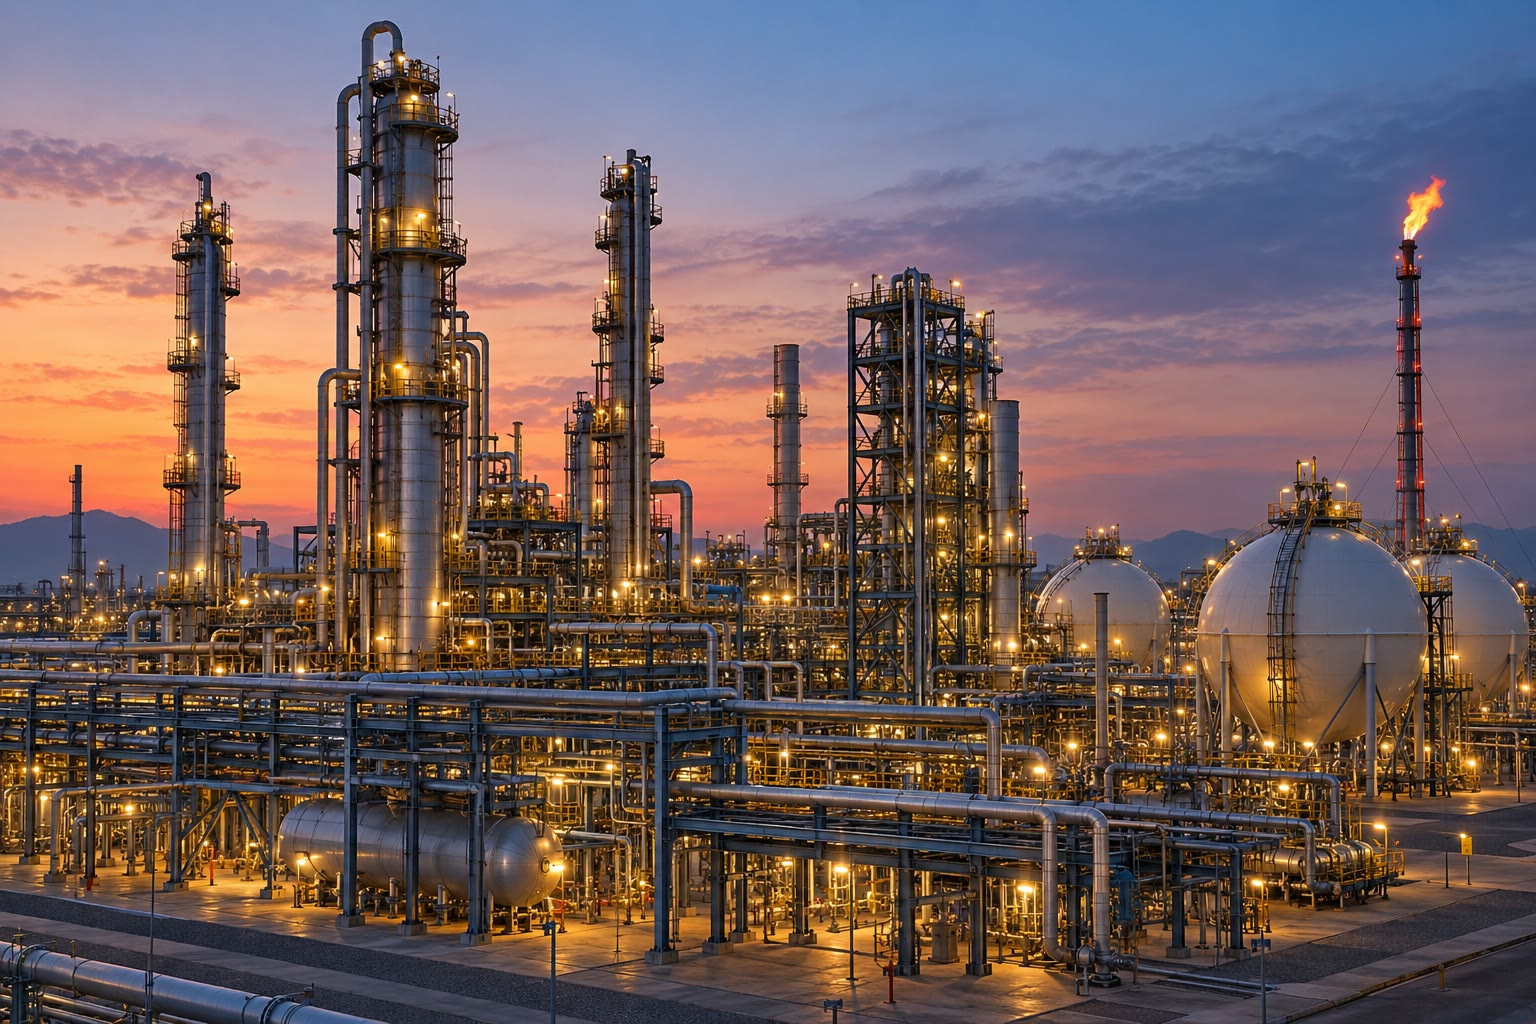
\includegraphics[width=0.6\linewidth]{images/book4/ai/b3-16-ammonia-plant.jpg}

{\small Une usine de synthèse de l'ammoniac. Le réacteur, en son cœur,
contient des tonnes de catalyseur au fer promu~; l'essentiel de l'usine
prépare le dihydrogène et recycle le gaz non converti.}
\end{omfigure}

\section{Observer les surfaces}

\begin{definition}[Spectroscopie de désorption thermique]\label{def:b3:surfaces-catalysis:tpd}
La \emph{spectroscopie de désorption thermique}\index{spectroscopie de desorption thermique@spectroscopie de désorption thermique}
chauffe à vitesse constante une surface portant un \omterm{def:b3:surfaces-catalysis:adsorption}{adsorbat} et enregistre
le gaz désorbé à l'aide d'un spectromètre de masse~; chaque état de
liaison donne un pic, dont la température croît avec son énergie
d'activation de \omterm{def:b3:surfaces-catalysis:adsorption}{désorption}.
\end{definition}

La position d'un pic de \omterm{def:b3:surfaces-catalysis:adsorption}{désorption} donne l'énergie de \omterm{def:b3:surfaces-catalysis:adsorption}{désorption} (pour
une \omterm{def:b3:surfaces-catalysis:adsorption}{désorption} d'ordre 1,
$E_d \approx RT_{\mathrm p}[\ln(\nu T_{\mathrm p}/\beta) - 3.64]$, avec
$\beta$ la vitesse de chauffage et $\nu \approx \qty{e13}{s^{-1}}$,
résultat admis), son aire la quantité adsorbée. La spectroscopie de
photoélectrons X (XPS) mesure les énergies de liaison des électrons de
cœur des atomes de surface, qui identifient les éléments et leurs états
d'oxydation dans les premiers nanomètres. Le microscope à \omterm{def:b3:quantum-model-systems:tunnelling}{effet tunnel}
déplace une pointe fine à quelques dixièmes de nanomètre au-dessus d'une
surface conductrice~; le courant tunnel
(\cref{ch:b3:quantum-model-systems}) diminue d'environ un ordre de
grandeur pour chaque \qty{0.1}{nm} de distance supplémentaire, si bien
que le maintenir constant pendant le balayage cartographie la surface
atome par atome.

\begin{inthelab}[Une mesure BET]
Environ \qty{0.2}{g} d'échantillon est pesé dans un tube de verre à
bulbe, dégazé pendant des heures sous vide entre 150 et
\qty{300}{\celsius}, pesé de nouveau, puis monté sur l'appareil, le bulbe
plongé dans un vase Dewar d'azote liquide. L'appareil admet le diazote
par petites doses et mesure la pression d'équilibre après chacune, en
déduisant la quantité adsorbée du bilan gazeux~; le volume mort du tube
est mesuré avec de l'hélium, qui ne s'adsorbe pas.
\end{inthelab}

\begin{safety}{\ghs[0.7cm]{GHS06}\ghs[0.7cm]{GHS07}\ghs[0.7cm]{GHS08}\ghs[0.7cm]{GHS09}}
% ledger: ghs4:V2O5, ghs4:Ni
Les catalyseurs métalliques réduits (nickel, palladium ou platine
finement divisés sur un support, fraîchement réduits sous dihydrogène)
peuvent s'enflammer au contact de l'air~: on les manipule sous gaz inerte
et on les passive avant de les stocker. Le nickel est un sensibilisant
cutané et un cancérogène suspecté~; l'oxyde de vanadium(V) est toxique
par inhalation et par ingestion et peut provoquer le cancer. Les poudres
de catalyseur sont pesées dans une enceinte ventilée.
\end{safety}

\begin{history}[Langmuir et le catalyseur de l'ammoniac]
Irving Langmuir, qui travaillait sur les ampoules électriques dans un
laboratoire industriel, établit son isotherme en 1916--1918 à partir de
l'idée que les gaz adsorbés forment une couche épaisse d'une seule
molécule, et reçut en 1932 le prix Nobel de chimie pour ses travaux de
chimie des surfaces. Quelques années plus tôt, Alwin Mittasch avait
organisé la recherche d'un catalyseur pratique pour l'ammoniac~: des
milliers de compositions furent essayées dans de petits réacteurs à
haute pression avant que soit retenu le catalyseur au fer promu, encore
utilisé aujourd'hui. Ce fut l'un des premiers criblages systématiques de
catalyseurs.
\end{history}

\section{Exercices}

\begin{exercise}[$\star$]\label{exo:b3:surfaces-catalysis:1}
Un gaz recouvre 40\,\% d'une surface de Langmuir sous \qty{2.0}{kPa}.
Calculer $K$ et le \omterm{def:b3:surfaces-catalysis:coverage}{taux de recouvrement} sous
\qty{10}{kPa}.
\end{exercise}

\begin{exercise}[$\star$]\label{exo:b3:surfaces-catalysis:2}
On mesure deux enthalpies d'\omterm{def:b3:surfaces-catalysis:adsorption}{adsorption} sur un métal~: $-20$ et
\qty{-150}{kJ/mol}. Laquelle correspond à une \omterm{def:b3:surfaces-catalysis:physi-chemi}{physisorption}, laquelle à
une \omterm{def:b3:surfaces-catalysis:physi-chemi}{chimisorption}~? Laquelle pourrait être dissociative~?
\end{exercise}

\begin{exercise}[$\star$]\label{exo:b3:surfaces-catalysis:3}
Dénombrer, par atome de surface, les sites sommets, pontés et creux d'une
face (100) et d'une face (111) d'un métal cubique à faces centrées.
\end{exercise}

\begin{exercise}[$\star$]\label{exo:b3:surfaces-catalysis:4}
Un catalyseur transforme \qty{3.0e-6}{mol} de réactif par gramme et par
seconde et porte
\qty{1.5e-5}{mol} de sites de surface par gramme. Calculer la fréquence
de cycles.
\end{exercise}

\begin{exercise}[$\star\star$]\label{exo:b3:surfaces-catalysis:5}
Le dihydrogène s'adsorbe de façon dissociative avec $\theta = 0.10$ sous \qty{1.0}{kPa}. Calculer $\theta$ sous \qty{4.0}{kPa}.
\end{exercise}

\begin{exercise}[$\star\star$]\label{exo:b3:surfaces-catalysis:6}
CO ($K = \qty{10}{kPa^{-1}}$) et \ce{O2} ($K = \qty{0.5}{kPa^{-1}}$, non
dissociatif dans ce modèle simple) sont en compétition pour les sites
d'une surface de platine sous 1.0 et \qty{5.0}{kPa}. Calculer les deux
\omterm{def:b3:surfaces-catalysis:coverage}{taux de recouvrement} et commenter la vitesse d'oxydation de CO.
\end{exercise}

\begin{exercise}[$\star\star$]\label{exo:b3:surfaces-catalysis:7}
Un \omterm{def:b3:surfaces-catalysis:coverage}{taux de recouvrement} atteint sous \qty{1.0}{kPa} à \qty{300}{K} exige
\qty{8.0}{kPa} à \qty{350}{K}. Calculer l'\omterm{def:b3:surfaces-catalysis:isosteric}{enthalpie isostérique
d'adsorption}.
\end{exercise}

\begin{exercise}[$\star\star$]\label{exo:b3:surfaces-catalysis:8}
% ledger: sa:N2.am, const:Vm1, const:NA
Un charbon actif a $v_{\mathrm m} = \qty{120}{cm^3.g^{-1}}$ (conditions
normales, 273.15 K et
\qty{101.325}{kPa}). Calculer sa surface BET.
\end{exercise}

\begin{exercise}[$\star\star$]\label{exo:b3:surfaces-catalysis:9}
La vitesse de $\ce{2 CO + O2 -> 2 CO2}$ sur le platine croît, passe par un
maximum puis décroît quand $p(\ce{CO})$
augmente à $p(\ce{O2})$ fixée. Quel mécanisme cela indique-t-il, et
pourquoi CO inhibe-t-il la réaction~?
\end{exercise}

\begin{exercise}[$\star\star\star$]\label{exo:b3:surfaces-catalysis:10}
Une réaction de surface a une énergie d'activation vraie de
\qty{100}{kJ/mol}~; le réactif a
$\Delta_{\mathrm{ads}}H = \qty{-60}{kJ/mol}$. Quelle énergie
d'activation mesure-t-on à faible et à fort \omterm{def:b3:surfaces-catalysis:coverage}{taux de recouvrement}~?
Esquisser $\ln r$ en fonction de $1/T$ sur un large domaine.
\end{exercise}

\begin{exercise}[$\star\star\star$]\label{exo:b3:surfaces-catalysis:11}
Le soufre s'adsorbe sur un catalyseur au nickel avec un \omterm{def:b3:surfaces-catalysis:coverage}{taux de
recouvrement} de 0.10 (atomes de soufre par Ni de surface), chaque atome
de soufre bloquant quatre sites. Quelle fraction de l'activité subsiste
pour une réaction qui exige un site libre~? Deux sites libres adjacents
(en supposant les sites bloqués répartis au hasard)~?
\end{exercise}

\begin{exercise}[$\star\star\star$]\label{exo:b3:surfaces-catalysis:12}
Pour la synthèse de l'ammoniac, trois métaux fixent l'azote atomique avec
des enthalpies de
$-150$, $-250$ et \qty{-400}{kJ/mol} (données de l'exercice). D'après le
\omterm{def:b3:surfaces-catalysis:sabatier}{principe de Sabatier}, lequel est probablement le meilleur catalyseur, et
qu'est-ce qui limite les deux autres~?
\end{exercise}

\section{Problème~: caractériser un catalyseur}

\begin{problem}[{Problème du week-end --- caractériser un catalyseur~: la
surface BET d'un catalyseur au platine supporté, sa dispersion
métallique et la taille de ses particules par chimisorption du
dihydrogène, et la fréquence de cycles d'une hydrogénation}]
\label{pb:b3:surfaces-catalysis:1}
% ledger: sa:N2.am, lat:Pt, aw:Pt, const:Vm1, const:NA
Un catalyseur contient 1.00\,\% en masse de platine sur alumine. Données
du problème~: isotherme de diazote à \qty{77}{K} (volumes ramenés aux
conditions normales, 273.15 K et
\qty{101.325}{kPa}, par gramme)~:
\begin{center}\small
\begin{tabular}{lcccccc}
\hline
$x = p/p^*$ & 0.05 & 0.10 & 0.15 & 0.20 & 0.25 & 0.30 \\
$v$ / \unit{cm^3.g^{-1}} & 41.2 & 46.1 & 51.1 & 54.1 & 58.9 & 62.9 \\ \hline
\end{tabular}
\end{center}
\ce{H2} chimisorbé sur le platine~: \qty{0.205}{cm^3} par gramme de
catalyseur. Une hydrogénation se déroule à \qty{2.0e-5}{mol} par gramme
de catalyseur et par seconde. Platine~: $M = \qty{195.08}{g/mol}$,
cubique à faces centrées,
$a = \qty{392.3}{pm}$~; volume molaire d'un gaz dans les conditions
normales \qty{22414}{cm^3/mol}~;
$a_{\mathrm m}(\ce{N2}) = \qty{0.162}{nm^2}$.

\medskip\noindent\textbf{Partie I --- Le tracé BET.}
\begin{enumerate}
  \item Pourquoi mesure-t-on l'isotherme à \qty{77}{K}~?
  \item Pourquoi n'utilise-t-on que les pressions relatives comprises
        entre 0.05 et 0.30~?
  \item Calculer $x/(v(1 - x))$ pour chaque point.
  \item La droite des moindres carrés a pour pente \num{0.02205} et pour
        ordonnée à l'origine \num{0.000180} (en
        \unit{g.cm^{-3}}). En déduire $v_{\mathrm m}$.
  \item En déduire $c$. Que signifie une grande valeur de $c$~?
  \item Pourquoi l'ordonnée à l'origine est-elle si mal déterminée, et
        cela compte-t-il pour $v_{\mathrm m}$~?
\end{enumerate}

\medskip\noindent\textbf{Partie II --- L'aire.}
\begin{enumerate}[resume]
  \item Calculer la quantité de diazote de la \omterm{def:b3:surfaces-catalysis:coverage}{monocouche} par gramme.
  \item Calculer la \omterm{def:b3:surfaces-catalysis:surface-area}{surface spécifique}.
  \item Quelle partie du solide fournit presque toute cette aire~?
  \item Pourquoi la méthode BET échoue-t-elle pour les solides
        microporeux comme les zéolithes~?
\end{enumerate}

\medskip\noindent\textbf{Partie III --- Dispersion et taille des particules.}
\begin{enumerate}[resume]
  \item Calculer la quantité d'atomes H chimisorbés par gramme.
  \item Calculer la quantité de platine par gramme.
  \item En déduire la dispersion.
  \item Calculer le volume par atome de Pt dans le massif.
  \item L'aire par atome de surface, moyennée sur les faces (111), (100) et
        (110), vaut \qty{0.0807}{nm^2}. Vérifier la valeur pour (111),
        $\frac{\sqrt3}{4}a^2$.
  \item Montrer que, pour des sphères, $d = 6v_{\mathrm{at}}/(a_{\mathrm{at}}D)$.
  \item Calculer le diamètre moyen des particules.
  \item Quelles hypothèses limitent ce résultat~?
\end{enumerate}

\medskip\noindent\textbf{Partie IV --- L'activité.}
\begin{enumerate}[resume]
  \item Calculer la fréquence de cycles par atome de Pt de surface.
  \item Calculer la vitesse par gramme de platine.
  \item Si les particules frittaient jusqu'à \qty{10}{nm} à fréquence de
        cycles constante, de quel facteur la vitesse par gramme
        diminuerait-elle~?
  \item Que révélerait une fréquence de cycles qui varie avec la taille
        des particules~?
  \item Pourquoi compare-t-on les catalyseurs par leur fréquence de
        cycles plutôt que par leur vitesse par gramme~?
  \item Énoncer le résultat~: le diamètre moyen des particules de platine.
\end{enumerate}
\end{problem}
